% Options for packages loaded elsewhere
\PassOptionsToPackage{unicode}{hyperref}
\PassOptionsToPackage{hyphens}{url}
\PassOptionsToPackage{dvipsnames,svgnames*,x11names*}{xcolor}
%
\documentclass[
  11pt,
  a4paper,
]{article}
\usepackage[]{mathpazo}
\usepackage{setspace}
\usepackage{amsmath}
\usepackage{ifxetex,ifluatex}
\ifnum 0\ifxetex 1\fi\ifluatex 1\fi=0 % if pdftex
  \usepackage[T1]{fontenc}
  \usepackage[utf8]{inputenc}
  \usepackage{textcomp} % provide euro and other symbols
  \usepackage{amssymb}
\else % if luatex or xetex
  \usepackage{unicode-math}
  \defaultfontfeatures{Scale=MatchLowercase}
  \defaultfontfeatures[\rmfamily]{Ligatures=TeX,Scale=1}
\fi
% Use upquote if available, for straight quotes in verbatim environments
\IfFileExists{upquote.sty}{\usepackage{upquote}}{}
\IfFileExists{microtype.sty}{% use microtype if available
  \usepackage[]{microtype}
  \UseMicrotypeSet[protrusion]{basicmath} % disable protrusion for tt fonts
}{}
\makeatletter
\@ifundefined{KOMAClassName}{% if non-KOMA class
  \IfFileExists{parskip.sty}{%
    \usepackage{parskip}
  }{% else
    \setlength{\parindent}{0pt}
    \setlength{\parskip}{6pt plus 2pt minus 1pt}}
}{% if KOMA class
  \KOMAoptions{parskip=half}}
\makeatother
\usepackage{xcolor}
\IfFileExists{xurl.sty}{\usepackage{xurl}}{} % add URL line breaks if available
\IfFileExists{bookmark.sty}{\usepackage{bookmark}}{\usepackage{hyperref}}
\hypersetup{
  pdftitle={A template for writing manuscripts in Rmarkdown},
  pdfauthor={Francisco Rodríguez-Sánchez1,2*; Second Author3},
  colorlinks=true,
  linkcolor=RoyalBlue,
  filecolor=Maroon,
  citecolor=Blue,
  urlcolor=RoyalBlue,
  pdfcreator={LaTeX via pandoc}}
\urlstyle{same} % disable monospaced font for URLs
\usepackage[margin=1in]{geometry}
\usepackage{longtable,booktabs}
\usepackage{calc} % for calculating minipage widths
% Correct order of tables after \paragraph or \subparagraph
\usepackage{etoolbox}
\makeatletter
\patchcmd\longtable{\par}{\if@noskipsec\mbox{}\fi\par}{}{}
\makeatother
% Allow footnotes in longtable head/foot
\IfFileExists{footnotehyper.sty}{\usepackage{footnotehyper}}{\usepackage{footnote}}
\makesavenoteenv{longtable}
\usepackage{graphicx}
\makeatletter
\def\maxwidth{\ifdim\Gin@nat@width>\linewidth\linewidth\else\Gin@nat@width\fi}
\def\maxheight{\ifdim\Gin@nat@height>\textheight\textheight\else\Gin@nat@height\fi}
\makeatother
% Scale images if necessary, so that they will not overflow the page
% margins by default, and it is still possible to overwrite the defaults
% using explicit options in \includegraphics[width, height, ...]{}
\setkeys{Gin}{width=\maxwidth,height=\maxheight,keepaspectratio}
% Set default figure placement to htbp
\makeatletter
\def\fps@figure{htbp}
\makeatother
\setlength{\emergencystretch}{3em} % prevent overfull lines
\providecommand{\tightlist}{%
  \setlength{\itemsep}{0pt}\setlength{\parskip}{0pt}}
\setcounter{secnumdepth}{-\maxdimen} % remove section numbering
\pagestyle{plain}
\usepackage{lineno} % add 
\linenumbers % turns line numbering on 

% Allowing for landscape pages
\usepackage{lscape}
\newcommand{\blandscape}{\begin{landscape}}
\newcommand{\elandscape}{\end{landscape}}

% Left justification of the text: see https://www.sharelatex.com/learn/Text_alignment
% \usepackage[document]{ragged2e} % already in the latex template
\newcommand{\bleft}{\begin{flushleft}}
\newcommand{\eleft}{\end{flushleft}}


% Add Supplementary Tables and Figures
% Code from https://stackoverflow.com/a/51337664
\newcommand{\beginsupplement}{
  \setcounter{table}{0}  
  \renewcommand{\thetable}{S\arabic{table}}
  \setcounter{figure}{0} 
  \renewcommand{\thefigure}{S\arabic{figure}}
}



\ifluatex
  \usepackage{selnolig}  % disable illegal ligatures
\fi
\newlength{\cslhangindent}
\setlength{\cslhangindent}{1.5em}
\newlength{\csllabelwidth}
\setlength{\csllabelwidth}{3em}
\newenvironment{CSLReferences}[2] % #1 hanging-ident, #2 entry spacing
 {% don't indent paragraphs
  \setlength{\parindent}{0pt}
  % turn on hanging indent if param 1 is 1
  \ifodd #1 \everypar{\setlength{\hangindent}{\cslhangindent}}\ignorespaces\fi
  % set entry spacing
  \ifnum #2 > 0
  \setlength{\parskip}{#2\baselineskip}
  \fi
 }%
 {}
\usepackage{calc}
\newcommand{\CSLBlock}[1]{#1\hfill\break}
\newcommand{\CSLLeftMargin}[1]{\parbox[t]{\csllabelwidth}{#1}}
\newcommand{\CSLRightInline}[1]{\parbox[t]{\linewidth - \csllabelwidth}{#1}\break}
\newcommand{\CSLIndent}[1]{\hspace{\cslhangindent}#1}

\title{A template for writing manuscripts in Rmarkdown}
\author{Francisco Rodríguez-Sánchez\textsuperscript{1,2}* \and Second Author\textsuperscript{3}}
\date{}

\begin{document}
\maketitle

\setstretch{2}
\small

\textsuperscript{1} Estación Biológica de Doñana (CSIC)

\textsuperscript{2} Universidad de Sevilla

\textsuperscript{3} Second Author affiliation

\texttt{*} Corresponding author: \href{mailto:example@example.com}{\nolinkurl{example@example.com}}

\normalsize

\vspace{1cm}
\hrule

Write your abstract here.

\vspace{3mm}
\hrule
\vspace{5mm}

\emph{Keywords}: Rmarkdown, reproducible science

\bleft
\newpage

\hypertarget{introduction}{%
\section{INTRODUCTION}\label{introduction}}

Write your introduction here.

You can \textbf{cite bibliography} like this (\protect\hyperlink{ref-Yan2011}{Yan and Gerstein 2011}, \protect\hyperlink{ref-Sutherland2011}{Sutherland et al. 2011}) if you provide a \texttt{BibTeX} file with references. You can also search for references on PubMed, DataCite or Crossref, cite by DOI, or read them from your Zotero library or a shared Zotero group (see \url{https://rstudio.github.io/visual-markdown-editing/\#/citations} and \url{https://rmarkdown.rstudio.com/authoring_bibliographies_and_citations.html} for more information).

You can also specify the desired output format for your bibliography (see \texttt{csl} field in the YAML above). Many different bibliography styles (CSL files) can be obtained at \url{https://zotero.org/styles} or \url{https://github.com/citation-style-language/styles}.

\hypertarget{methods}{%
\section{METHODS}\label{methods}}

\hypertarget{study-area}{%
\subsection{Study Area}\label{study-area}}

We worked in a \textbf{beautiful} place with lots of trees, like \emph{Quercus suber} and \emph{Laurus nobilis}.

\hypertarget{data-collection-and-analysis}{%
\subsection{Data collection and analysis}\label{data-collection-and-analysis}}

We applied a linear model where

\[
y_{i} = \alpha + \beta*x_{i} 
\]

We used the statistical language \texttt{R} (\protect\hyperlink{ref-R_Core_Team_2020}{R Core Team 2020}) for all our analyses. These were implemented in dynamic rmarkdown documents using \texttt{knitr} (\protect\hyperlink{ref-Xie_2014}{Xie 2014}, \protect\hyperlink{ref-Xie_2015}{2015}, \protect\hyperlink{ref-Xie_2021}{2021}) and \texttt{rmarkdown} (\protect\hyperlink{ref-Xie_2018}{Xie et al. 2018}, \protect\hyperlink{ref-Xie_2020}{2020}, \protect\hyperlink{ref-Allaire_2021}{Allaire et al. 2021}) packages. All the multilevel models were fitted with \texttt{lme4} (\protect\hyperlink{ref-Bates_2015}{Bates et al. 2015}).

\hypertarget{results}{%
\section{RESULTS}\label{results}}

Trees in forest \emph{A} grew taller than those in forest \emph{B} (mean height: 25 versus 13 m).

And many more cool results that get updated dynamically, e.g.~see Table \ref{tab:Table-mtcars} and Fig. \ref{fig:scatterplot}. Note Tables and Figures are \textbf{cross-linked and numbered automatically}. They could also appear in the middle of the document, not necessarily at the end.

See also Fig. \ref{fig:SupplFig} and Table \ref{tab:SupplTable} in the Supplementary Material.

\hypertarget{discussion}{%
\section{DISCUSSION}\label{discussion}}

Discuss.

\hypertarget{conclusions}{%
\section{CONCLUSIONS}\label{conclusions}}

Wrap up

\hypertarget{acknowledgements}{%
\section{ACKNOWLEDGEMENTS}\label{acknowledgements}}

On the shoulders of giants.

\hypertarget{references}{%
\section{REFERENCES}\label{references}}

\hypertarget{refs}{}
\begin{CSLReferences}{1}{0}
\leavevmode\hypertarget{ref-Allaire_2021}{}%
Allaire, J., Y. Xie, J. McPherson, J. Luraschi, K. Ushey, A. Atkins, H. Wickham, J. Cheng, W. Chang, and R. Iannone. 2021. Rmarkdown: Dynamic documents for r.

\leavevmode\hypertarget{ref-Bates_2015}{}%
Bates, D., M. Mächler, B. Bolker, and S. Walker. 2015. Fitting linear mixed-effects models using {lme4}. Journal of Statistical Software 67:1--48.

\leavevmode\hypertarget{ref-R_Core_Team_2020}{}%
R Core Team. 2020. R: A language and environment for statistical computing. R Foundation for Statistical Computing, Vienna, Austria.

\leavevmode\hypertarget{ref-Sutherland2011}{}%
Sutherland, W. J., D. Goulson, S. G. Potts, and L. V. Dicks. 2011. Quantifying the impact and relevance of scientific research. PLoS ONE 6:e27537.

\leavevmode\hypertarget{ref-Xie_2014}{}%
Xie, Y. 2014. Knitr: A comprehensive tool for reproducible research in {R}. \emph{in} V. Stodden, F. Leisch, and R. D. Peng, editors. Implementing reproducible computational research. Chapman; Hall/CRC.

\leavevmode\hypertarget{ref-Xie_2015}{}%
Xie, Y. 2015. Dynamic documents with {R} and knitr. 2nd edition. Chapman; Hall/CRC, Boca Raton, Florida.

\leavevmode\hypertarget{ref-Xie_2021}{}%
Xie, Y. 2021. Knitr: A general-purpose package for dynamic report generation in r.

\leavevmode\hypertarget{ref-Xie_2018}{}%
Xie, Y., J. J. Allaire, and G. Grolemund. 2018. R markdown: The definitive guide. Chapman; Hall/CRC, Boca Raton, Florida.

\leavevmode\hypertarget{ref-Xie_2020}{}%
Xie, Y., C. Dervieux, and E. Riederer. 2020. R markdown cookbook. Chapman; Hall/CRC, Boca Raton, Florida.

\leavevmode\hypertarget{ref-Yan2011}{}%
Yan, K.-K., and M. Gerstein. 2011. The spread of scientific information: Insights from the web usage statistics in PLoS article-level metrics. PLoS ONE 6:e19917.

\end{CSLReferences}

\eleft

\clearpage

\listoftables

\newpage

\begin{table}

\caption{\label{tab:Table-Iris}A glimpse of the famous Iris dataset.}
\centering
\begin{tabular}[t]{rrrrl}
\toprule
Sepal.Length & Sepal.Width & Petal.Length & Petal.Width & Species\\
\midrule
5.1 & 3.5 & 1.4 & 0.2 & setosa\\
4.9 & 3.0 & 1.4 & 0.2 & setosa\\
4.7 & 3.2 & 1.3 & 0.2 & setosa\\
4.6 & 3.1 & 1.5 & 0.2 & setosa\\
5.0 & 3.6 & 1.4 & 0.2 & setosa\\
\addlinespace
5.4 & 3.9 & 1.7 & 0.4 & setosa\\
\bottomrule
\end{tabular}
\end{table}

\clearpage

\begin{table}

\caption{\label{tab:Table-mtcars}Now a subset of mtcars dataset.}
\centering
\begin{tabular}[t]{lrrrrrrrrrrr}
\toprule
  & mpg & cyl & disp & hp & drat & wt & qsec & vs & am & gear & carb\\
\midrule
Merc 280 & 19.2 & 6 & 167.6 & 123 & 3.92 & 3.440 & 18.30 & 1 & 0 & 4 & 4\\
Merc 280C & 17.8 & 6 & 167.6 & 123 & 3.92 & 3.440 & 18.90 & 1 & 0 & 4 & 4\\
Merc 450SE & 16.4 & 8 & 275.8 & 180 & 3.07 & 4.070 & 17.40 & 0 & 0 & 3 & 3\\
Merc 450SL & 17.3 & 8 & 275.8 & 180 & 3.07 & 3.730 & 17.60 & 0 & 0 & 3 & 3\\
Merc 450SLC & 15.2 & 8 & 275.8 & 180 & 3.07 & 3.780 & 18.00 & 0 & 0 & 3 & 3\\
\addlinespace
Cadillac Fleetwood & 10.4 & 8 & 472.0 & 205 & 2.93 & 5.250 & 17.98 & 0 & 0 & 3 & 4\\
Lincoln Continental & 10.4 & 8 & 460.0 & 215 & 3.00 & 5.424 & 17.82 & 0 & 0 & 3 & 4\\
\bottomrule
\end{tabular}
\end{table}

\clearpage

\listoffigures

\newpage

\begin{figure}
\centering
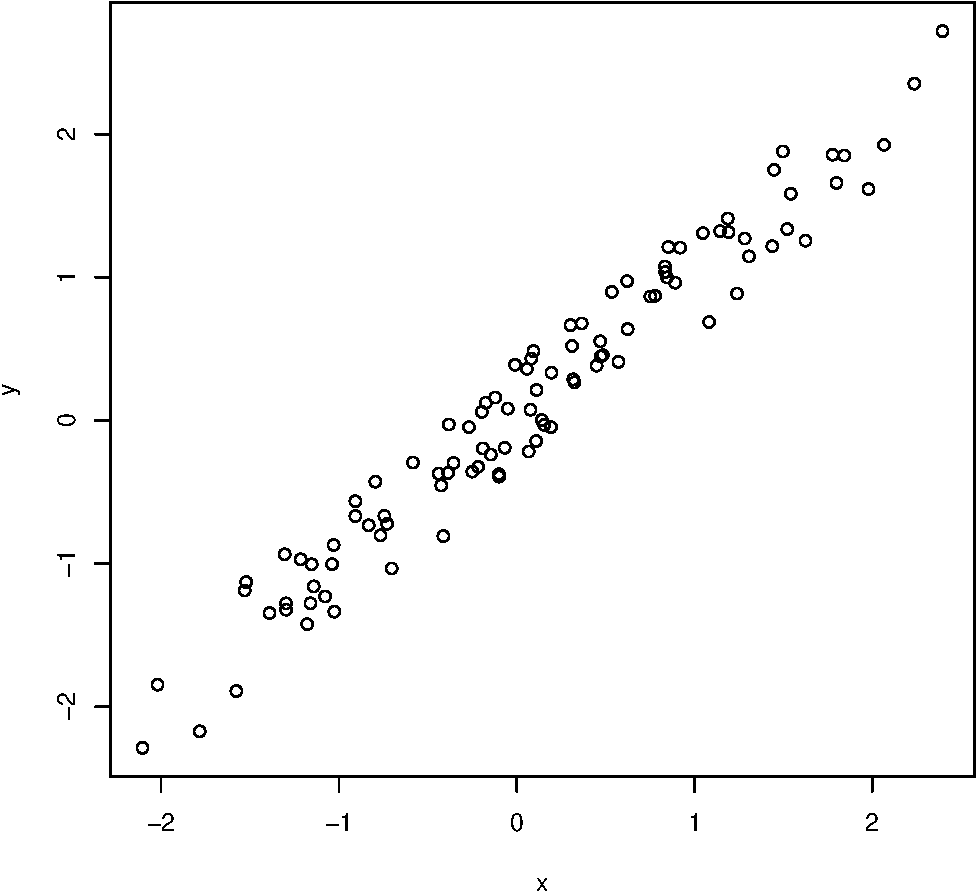
\includegraphics{output/figures/scatterplot-1.pdf}
\caption{\label{fig:scatterplot}Just my first figure with a very fantastic caption.}
\end{figure}

\newpage

\blandscape

\begin{figure}
\centering
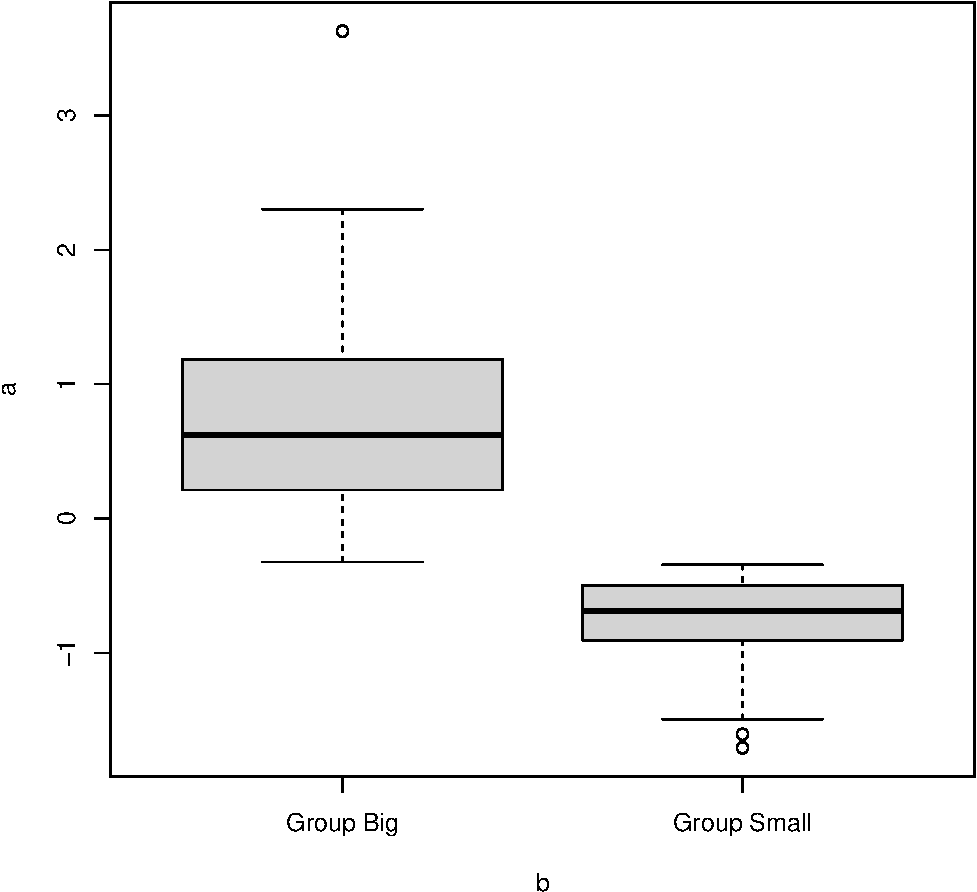
\includegraphics{output/figures/Fig-landscape-1.pdf}
\caption{\label{fig:Fig-landscape}Second figure in landscape format.}
\end{figure}

\elandscape

\clearpage

\hypertarget{supplementary-material}{%
\section*{SUPPLEMENTARY MATERIAL}\label{supplementary-material}}
\addcontentsline{toc}{section}{SUPPLEMENTARY MATERIAL}

\beginsupplement

\clearpage

\begin{table}

\caption{\label{tab:SupplTable}A supplementary table.}
\centering
\begin{tabular}[t]{rrrrl}
\toprule
Sepal.Length & Sepal.Width & Petal.Length & Petal.Width & Species\\
\midrule
5.1 & 3.5 & 1.4 & 0.2 & setosa\\
4.9 & 3.0 & 1.4 & 0.2 & setosa\\
4.7 & 3.2 & 1.3 & 0.2 & setosa\\
4.6 & 3.1 & 1.5 & 0.2 & setosa\\
5.0 & 3.6 & 1.4 & 0.2 & setosa\\
\addlinespace
5.4 & 3.9 & 1.7 & 0.4 & setosa\\
\bottomrule
\end{tabular}
\end{table}

\clearpage

\begin{figure}
\centering
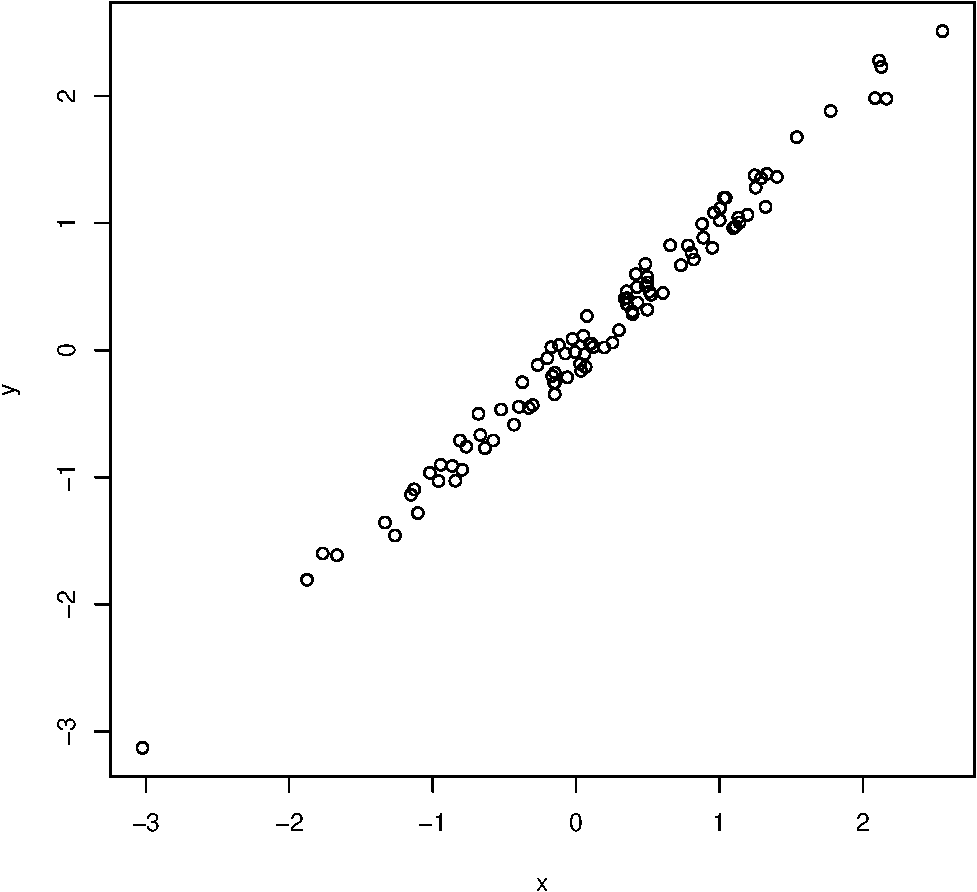
\includegraphics{output/figures/SupplFig-1.pdf}
\caption{\label{fig:SupplFig}A Supplementary Figure.}
\end{figure}

\newpage

\end{document}
